
	I also tried to normalize $M_n$ using theoretical expressions
	of the mean and variance. For the mean, the first order expression
	
	\centers{$E_n \sim \f{nh}{\log_2(n)}$}
	
	\noindent
	is, under $n\leq 10^6$, not sufficient to center the distribution. I conducted a numerical analysis
	of the difference between this expression and the empirical mean for growing 
	values of $n$. In particular, here is how their difference, in black, compares with
	different approximation functions 
	
	
	  \begin{figure}[H]
		\centering
        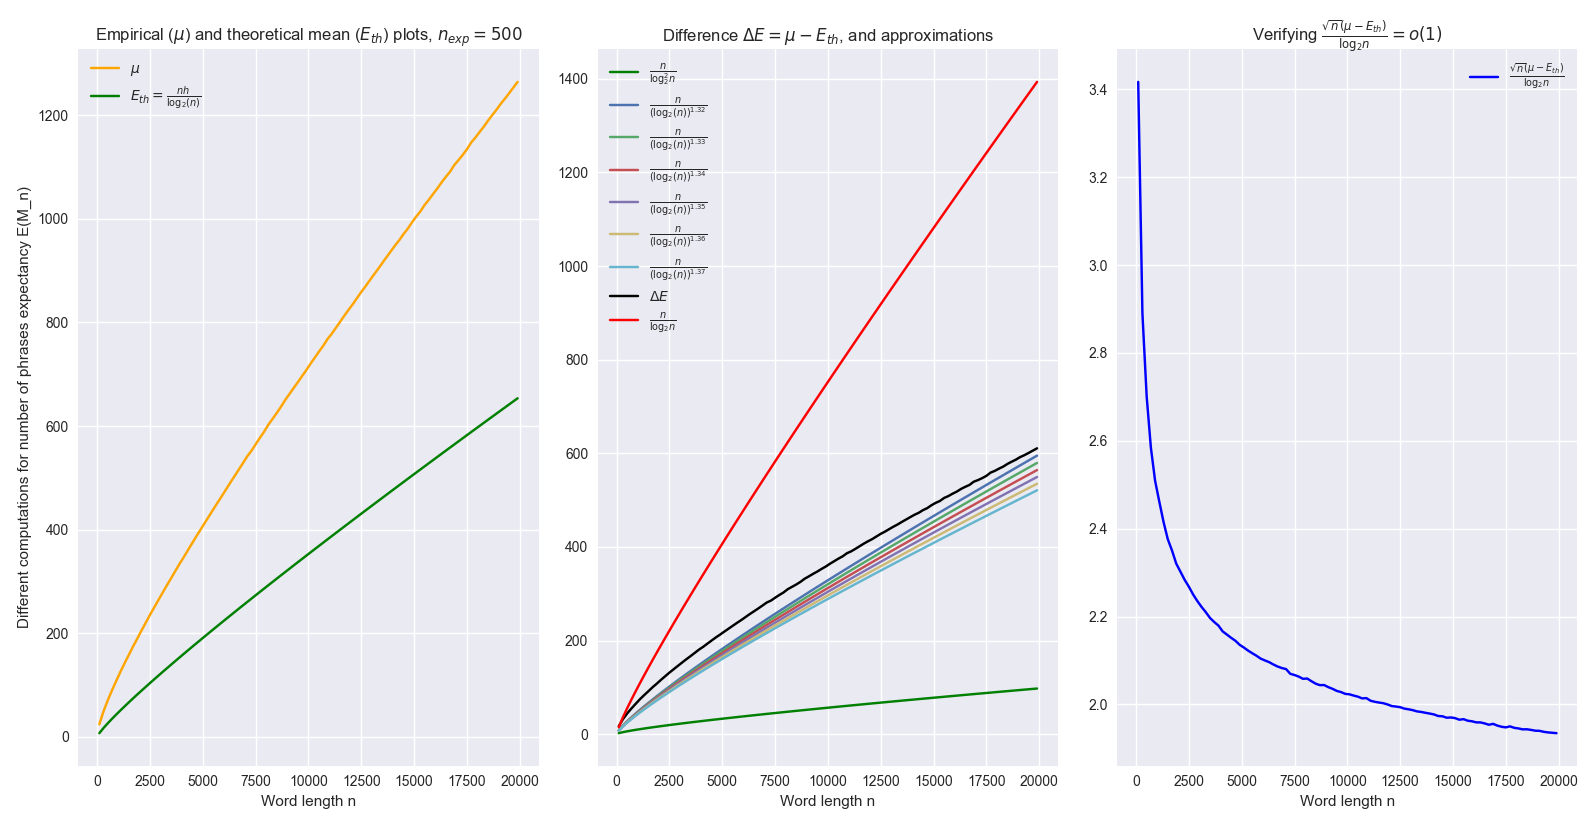
\includegraphics[width = 5cm,
        				    trim = 14cm 0 13cm 1.5cm,
								clip=true]{./figs/mean_analysis_2e4_500.png}
		\caption{Difference $\mu - \f{nh}{\log_2(n)}$ and approximation plots.}	
	  \end{figure}
	
	\noindent
	This is not troubling as it was already predicted in the formula:
	
	\centers{$E_n = 	\f{nh}{\log_2(n)} + \mathcal{O} \pa{ \f{n}{\log_2(n)} }$}
